\documentclass[]{report}
\usepackage{ucs}
\usepackage[latin1]{inputenc}
\usepackage[english]{babel}
\usepackage{amsmath}
\usepackage{marvosym}
%\usepackage{hyperref}
\usepackage[colorlinks=true,
            linkcolor=black,
            urlcolor=blue,
            citecolor=black]{hyperref}
\usepackage{breakurl}
\usepackage{fancyhdr}
\usepackage{graphicx}
\usepackage{float}
\usepackage[margin=2.7cm]{geometry}
\pagestyle{fancy}
\usepackage{subfig}
\usepackage{color, colortbl}
\usepackage{extraplaceins}
 

\fancyhead{}

\lhead{Advanced Natural Language Processing}
\chead{}
\rhead{}
\lfoot{
\includegraphics[scale=0.2]{img/upc}}
\cfoot{\thepage}

% Title Page
\title{Demonym gazetteer}
\date{29\textsuperscript{th}, May 2014}
\author{Alex Pardo and David Sanchez}


\begin{document}
\maketitle

\tableofcontents

\newpage

\section{Introduction}

Demonym or gentilic, is a term for the residents of a locality. How to generate the demonym from a country or city is not an easy task, and in order to automatize this process we are going to built a system which it is capable to do this automatically. The next document will show the description of the problem, our system approach, the evaluation and the discussions of the results. Finally, we will explain some possible improvements in our work as a future work.

\section{Attached files}

Identifiers of the attached files (classes, functions and script .py files and
data files when needed)

\section{Description of the problem}

As the document mentions in the introduction, the generation of the demonym from a location like country or city it is not a easy task. Exist a lot of possible rules and different cases. 
\\\\Some examples of this process are:
\begin{itemize}
\item Africa -- African
\item Croatia -- Croatian (also "Croat")
\item North / South Korea -- North / South Korean
\item Hanoi (Vietnam) -- Hanoian
\item Iran -- Iranian (also "Irani" or "Persian")
\item Florence -- Florentine (also Latin "Florentia")
\item Ann Arbor -- Ann Arborite
\item Israel -- Israelite (also "Israeli")
\item Netherlands -- Netherlander
\end{itemize}

For instance, as the examples of the above show, some demonyms are simple a process in which is needed to add ending letters in the original country or city. However, the irregular cases difficult the process to build the system because others constructions are based in delete some letters in the original word and add some ending new letters. Also, other problem to face is that some countries and cities have more than one demonym and this fact difficult the process to build a robust system. 

\newpage
\section{Approach}



Our system follows the general flow in this type of systems which it is based on two phases: training and test [\ref{Main architecture of our system.}]. The training test is the part in which the system download demonyms examples from the Wikipedia which they are pairs with country or city plus the demonym. 

%Architecture of the system
\begin{figure}[htb!]
\centering
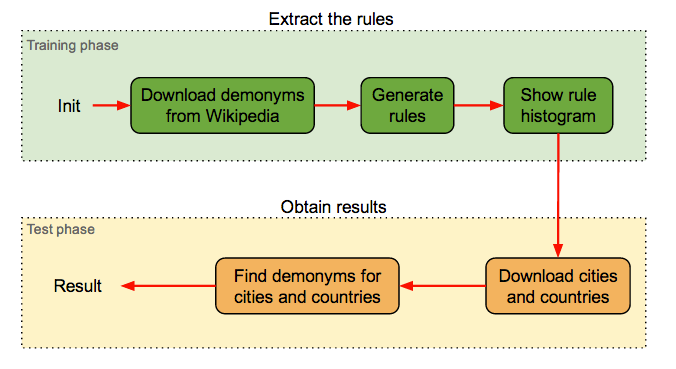
\includegraphics[scale=0.5]{img/architecture}
\caption{Main architecture of our system.}
\label{Main architecture of our system.}
\end{figure}

%Histogram figure
\begin{figure}[htb!]
\centering
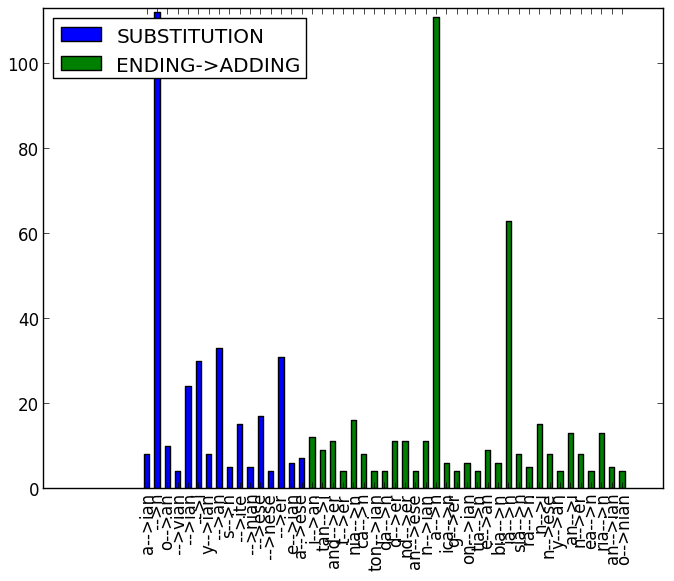
\includegraphics[scale=0.6]{img/rules}
\caption{Histogram of the rules.}
\label{Histogram of the rules.}
\end{figure}

In this moment, the system build and extract two different types of rules:
\begin{itemize}
\item Ending with this letters and transform or add new letters.
\item Delete this letters and add this.
\end{itemize}
An example of this two types of rules could be the Africa - African. From this example the system will built these rules:
\begin{itemize}
\item "a" - "an"
\item " " - "n"
\end{itemize}
The system construct all these types of rules for all the examples extracted from Wikipedia and build a graphical representation with histograms [\ref{Histogram of the rules.}]. The histogram filter the rules which they occurs rarely and it only shows the most popular rules.
\\\\The second phase is the test phase. First, the system download new countries and cities names (without demonym). The idea is based on generate automatically for each country or city its demonym. For do this, the system uses the rules knowledge (generated in the first step) and uses the most probable combination of the two different types of rules.

%IMPORTANT:
%A description of the approach used for solving the problem. It is
%important to argument why this approach has been followed against the
%possible alternatives.

\section{Evaluation}

The evaluation performed

\section{Discussion}

A discussion of the results

\section{Future work}

A proposal of possible improvements


\end{document}          
